\section{Results and Discussion}
\label{sec:discussion}

% <intro>

% Network
\subsection{Network structure}
At the beginning of the simulation, users are not connected: the social network starts in an empty state.
The network structure emerges over time, based on the interactions of the individuals: each time an agent interacts with another user, for instance by reading a post, it can decide to follow the author.
This mechanism replicates a realistic dynamic of the evolution of the network, which evolves according to the preferences and behavior of the agents.

\medskip
In Figure \ref{fig:network_structure} there are four examples of final networks generated by simulations with the default recommender system, but with different levels of misinformation.

Nodes are colored according to the supported coalition, while the bold borders indicate misinformation agents.
The network is not split into isolated groups: agents connect not only with members of the same coalition, but also with users from opposing coalitions, including misinformation agents.
This suggests that, at a structural level, the interaction among different groups are present even with users producing misleading content.

Moreover, some nodes look bigger, due to the higher number of connections they have.
This is valid also for some misinformation agents, confirming that they can have a realistic behavior and become central in the network.

\begin{figure}[h]
    \centering
    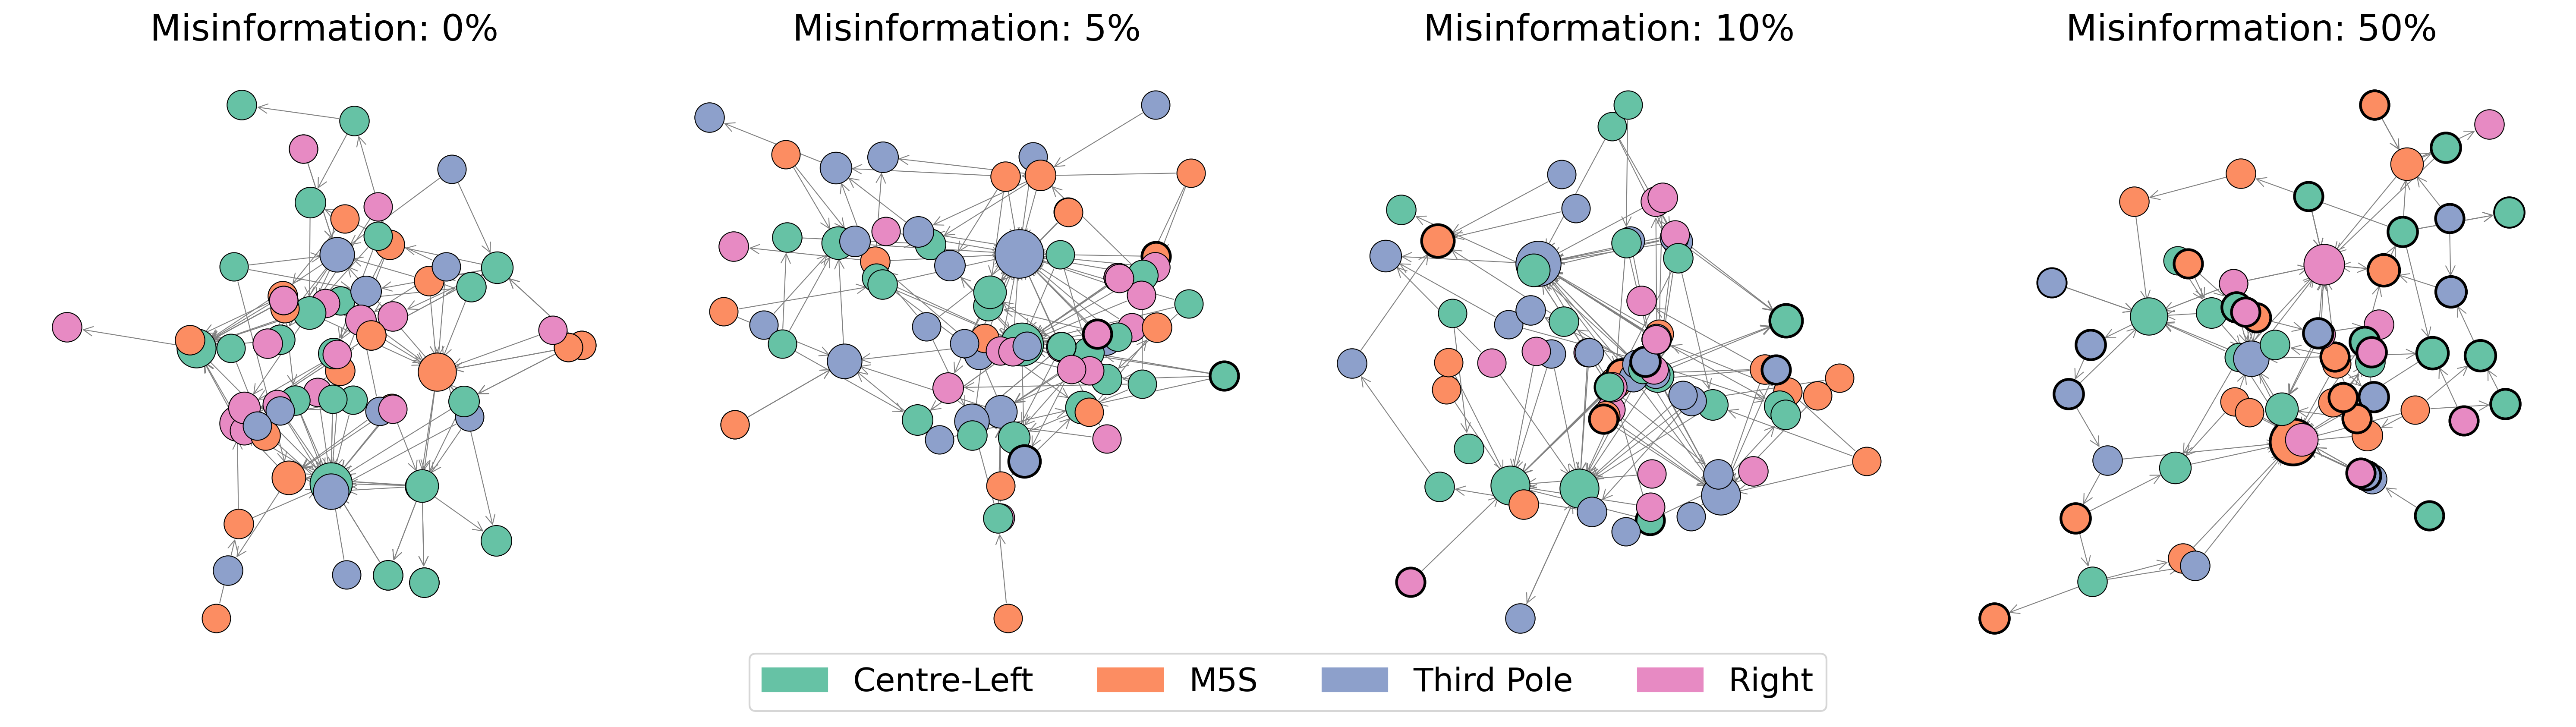
\includegraphics[width=1\linewidth]{Images/Network/graphs_DefaultRecSys.png}
    \caption{Final structure of the social network in four simulations with different levels of misinformation. 
    Nodes are agents, colored according to the supported coalition; the bold borders indicate misinformation agents. 
    The dimension of the nodes indicates the number of connections of an agent.
    The connections in the network are both in and out coalition, including misinformation agents.}
    \label{fig:network_structure}
\end{figure}


% evoluzione della rete (?)


% Opinion
\subsection{Opinion evolution}
One of the main aspects of the simulations is the evolution of opinions over time, which can be observed making a distinction for each topic and coalition.
Fig \ref{fig:opinion_evolution} shows the opinion evolution over virtual days, with a 95\% confidence interval, on each setup.
The plots on the top represent the score directly assigned by LLMs, while the ones on the bottom show the score computed with traditional opinion dynamic models.

Comparing the two score models highlights a high coherency in the trends: both scores evolves with the same behavior, and with similar mean values.
This suggests that LLMs are able to effectively replicate the opinions updates at the population level, as the observed behavior is close to that of established models in literature. Therefore, LLMs represent a valid approach in complex scenarios.

Across all topics, it's possible to observe a progressive convergence of opinions toward neutral values, indicating that agents trend to reduce their polarization over time.
It would be interesting to extend the duration of the simulations, as it would allow to determine if this trend persists or stabilizes.

Moreover, the general trend is the same even in different setups (with varying misinformation levels and different recommender systems), confirming the validity of these observations.

\begin{figure}[h]
    \centering
    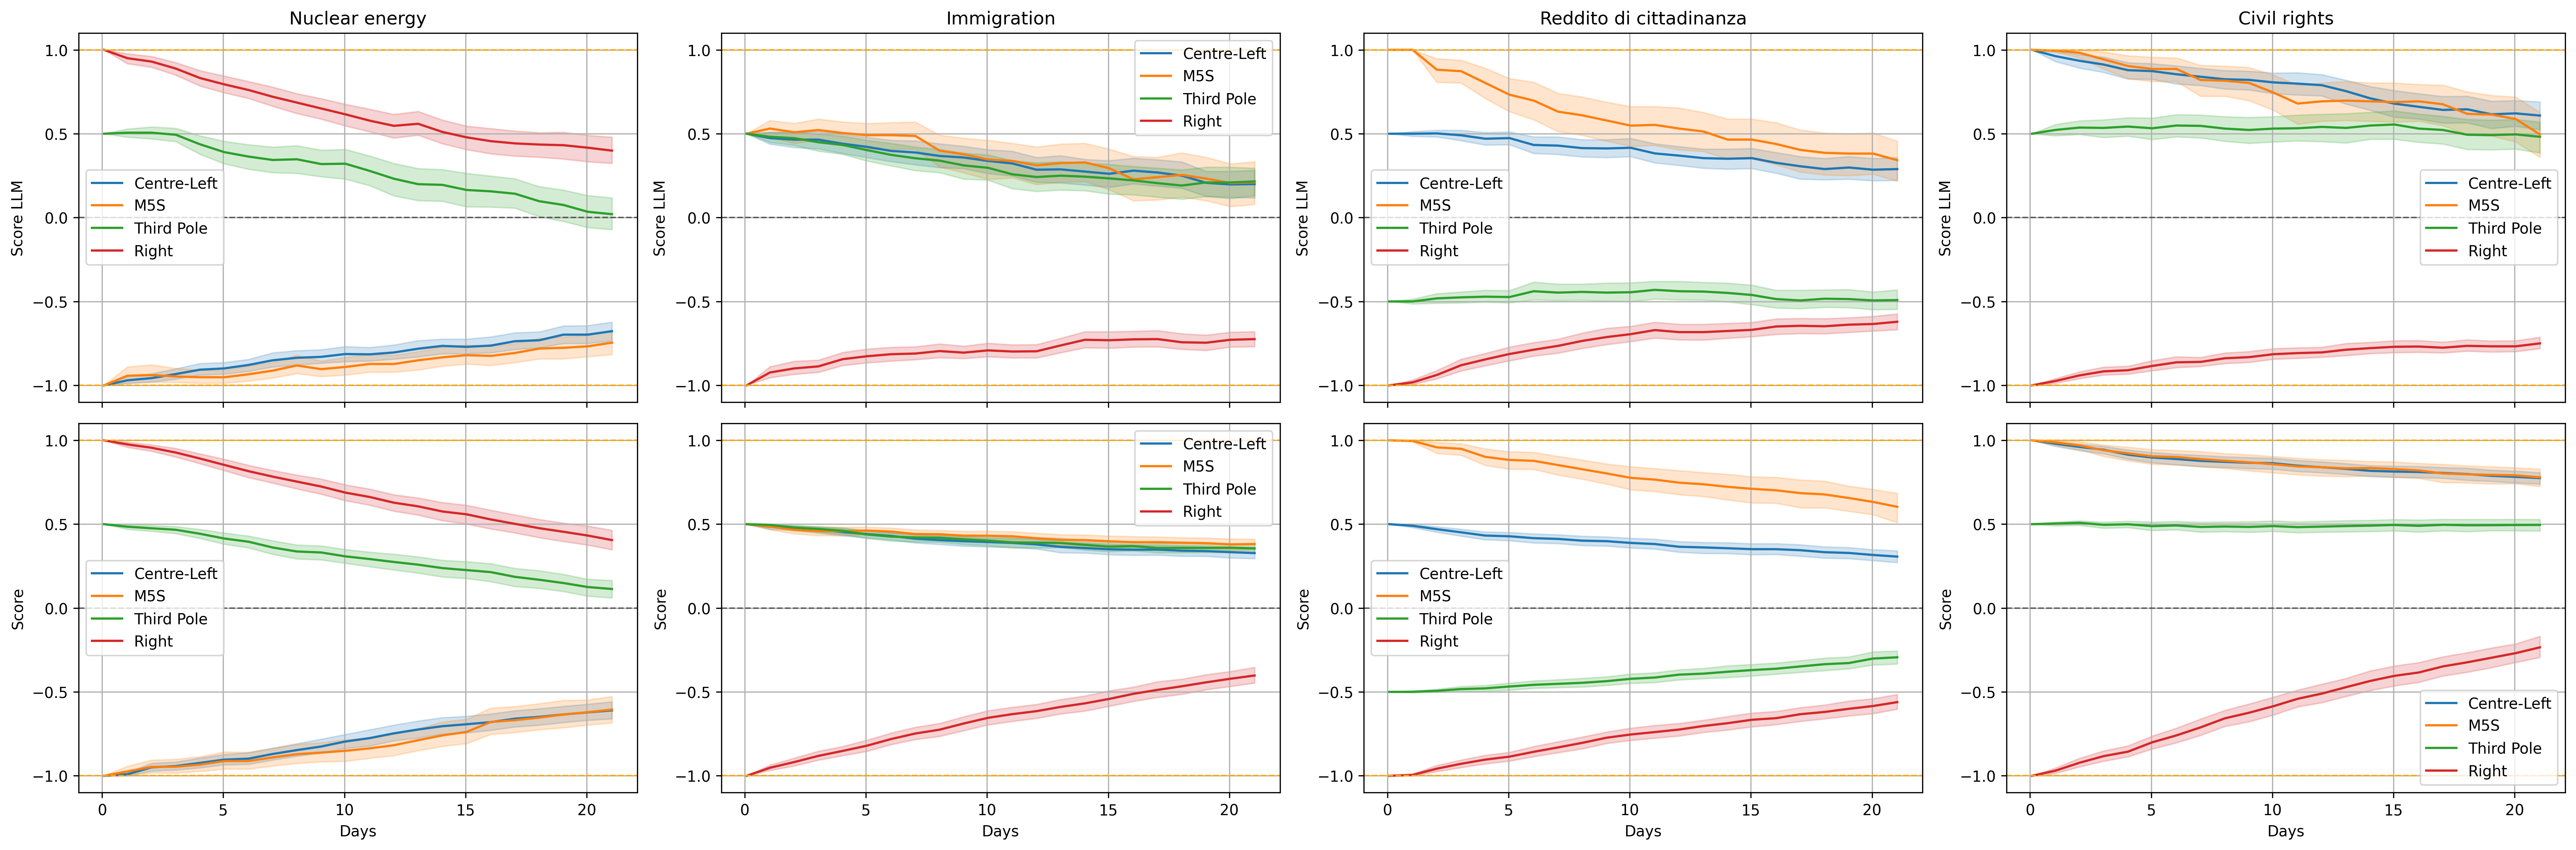
\includegraphics[width=1\linewidth]{Images/Opinions/d21a100m00d_DefaultRecSys.png}
    \caption{Evolution of opinion for each topic, comparing LLM-assigned score (\textit{score\_llm}, top row) and the one assigned by a traditional model (\textit{score}, bottom row).
    Each line represents a coalition, with a 95\% confidence interval.
    This figure is based on the runs for a single setup, but the trend is consistent with the other scenarios.}
    \label{fig:opinion_evolution}
\end{figure}


% ridge opinion shift by coalition




% misinformation

% toxicity analysis (in-out diff vs real data, post vs comment distributions)


% Recsys
\subsection{Content Recommendation Algorithms}
A comparison of the two content recommendation algorithms on the previously presented plots doesn't highlight any significant difference.
This happens because, at the beginning of the simulation, agents are not connected, so the network is empty.
Therefore, the used recommended system, \textit{ReverseChronoFollowersPopularity}, which should promote popular content from followers, doesn't have enough information to provide the best content.
In this initial phase, its behavior is similar to \textit{ContentRecSys}, the algorithm that suggests random content.

As a result, the different effects of the recommendation systems cannot emerge in the first few virtual days, and the dynamics produced by the two approaches are the same.
To see a real impact of the different recommender systems, simulations should run on a longer virtual time, or a network should be initialized with preexisting connections, providing a complete context of the initial user preferences.

This would allow a better evaluation of the impact of content selection on social networks.